

\chapter{Objects and experiments}

During the~course of~doctoral studies author has conducted his research based on~data acquired on~various types of~mining machines at~various stages of~the~production process. Considered objects included static machines (e.g. gearboxes and electric engines of~belt conveyors, bearings of~crusher shaft, belt conveyor drive pulley and oil rig gas compressors) as~well as~mobile ones (Load-Haul-Dump machines, haulage trucks, roadheader). Every object has its specific features and is~influenced differently by~the~operational and environmental conditions. Moreover, objects suffer differently from degradation processes specific to~their type.

\section{Objects of~interest for vibration data analysis}

Measurements on~regarded objects were performed using different data acquisition systems. This way, it~was possible for the~author to~acquire the~experience regarding the~analysis of~vibration signals that have different parameters. The most important acquisition systems for the~purpose of~author's work were:

\begin{itemize}
  \item \textbf{DiagManager}: portable 4-channel data acquisition system designed by~specialists from the~Faculty of~Geoengineering, Mining and Geology for KGHM. Used sampling frequency: 17 kHz 
  \item \textbf{Br{\"u}el \& Kjaer Pulse}: 7-channel portable data acquisition system. Used sampling frequency: 8192 Hz, 16384 Hz
  \item \textbf{NI-DAQ}: portable 2-channel data acquisition system based on~NI-DAQ data acquisition card and SignalExpress environment from National Instruments. Used sampling frequency: 25 kHz.
  \item \textbf{Pr{\"u}ftechnik}: bulit-in data acquisition system. Used sampling frequency: 19200 Hz.
  \item \textbf{EC Group}: bulit-in live monitoring system. Used sampling frequency: 24 kHz.
\end{itemize}

Failures encountered in~investigated machines contained meshing degradation on~the~gear wheel of~the~first shaft and tooth breakage on~the~gear wheel of~the~second shaft.

% Vibrations belong to~the~class of~fast-changing processes that require high sampling frequency for proper data acquisition. Taking advantage of~relatively fast sampling of~measured signals, one can perform certain types of~analysis, that capitalize on~the~small impact of~missing information. For signal processing tasks related to~damage detection and diagnostics in~general, methods of~favor include i.e. spectral-related analysis. Frequency-related methods also happen to~be very suitable for machine diagnostics, hence frequencies (or periods) that are present in~the~acquired vibration signals are directly related to:

% \begin{itemize}
%   \item Expected cycles related to~normal operation of~the~machine;
%   \item Periodic or otherwise cyclic components related to~local damage that occurred on~one of~the~elements of~the~machine.
% \end{itemize}

% Such an~assumption is~very promising, especially considering that machines with rotating elements are subjects of~the~majority of~the~analytical methods described in~this thesis.

\subsection{Gearbox in~belt conveyor drive}

In case of~the~belt conveyor drive unit the~purpose of~the~diagnostic experiment was to~acquire vibration signal from the~heavy-duty gearbox operating in~the~driving station (see Fig. \ref{fig:obj_gear}). 

% \begin{figure}[ht!]
% \centering
% 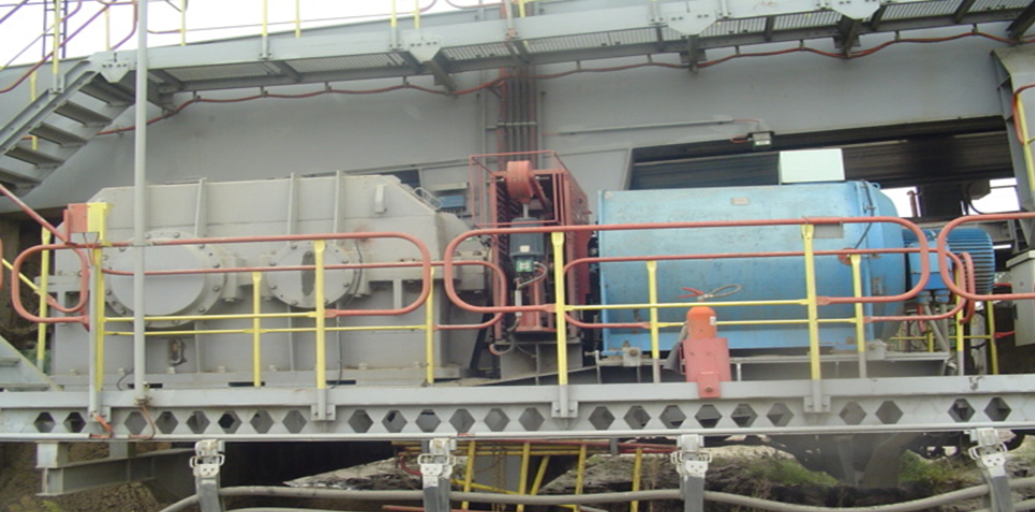
\includegraphics[width=0.7\textwidth]{wykresy/obj_gear.png}
% \caption{Two-stage gearbox operating in~the~driving station}
% \label{fig:obj_gear}
% \end{figure}

\begin{figure}[!ht]
 \centering
 \begin{subfigure}
   \centering
   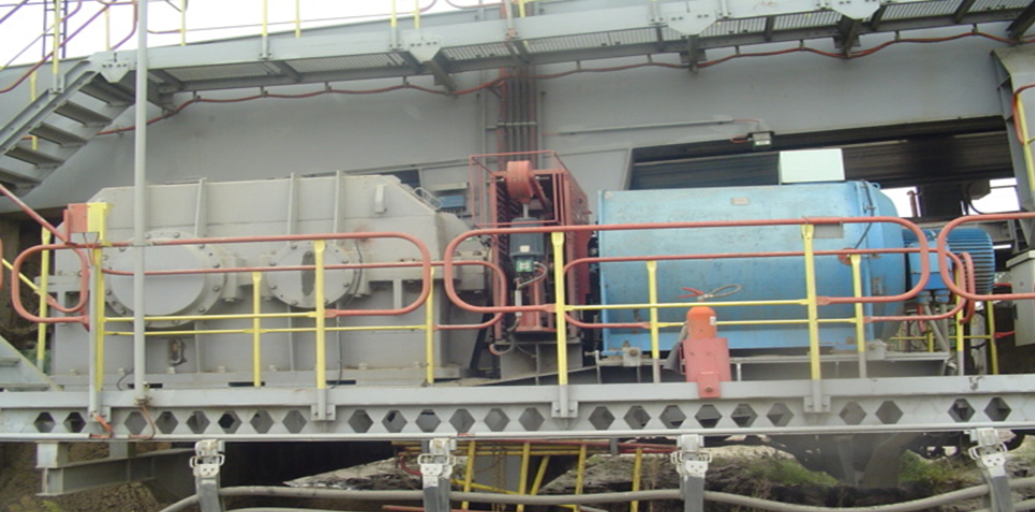
\includegraphics[width=0.48\textwidth]{wykresy/obj_gear.png}
 \end{subfigure}
 \begin{subfigure}
   \centering
		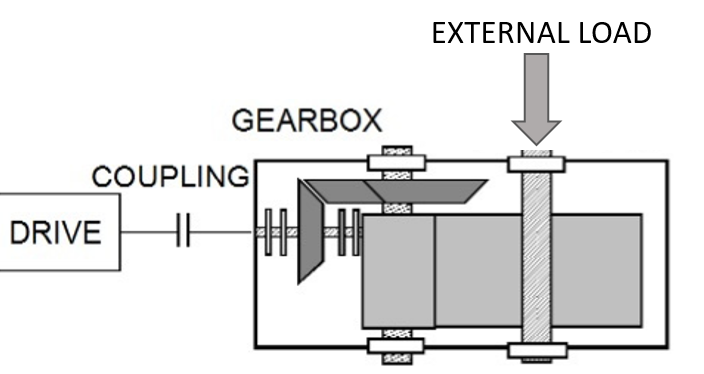
\includegraphics[width=0.48\textwidth]{wykresy/gb_sch2.png}
 \end{subfigure}
 \caption{Two-stage gearbox (left panel) and simplified schematic of~driving station (right panel)}
 \label{fig:obj_gear}
\end{figure}



Depending on~the~design (required power for driving of~belt conveyor), belt conveyor driving station might consist of~one up to~four drive units with 630 or 1000 [kW] power each. In this case a~two-stage gearbox has been diagnosed, with conical stage at~the~input and cylindrical one on~the~output. Characteristic frequencies present in~the~operation of~the~machine are shown in~Table \ref{tab: obj_gear}.

\begin{table}
	\begin{center}
		\begin{tabular}{|c|l|l|l|}
			
			\hline
			No & Notation & Description & Value/unit \\ \hline
			1 & $f_{01}=\frac{n_1}{60}$ & Rotational frequency of~the~first shaft & 16.58 Hz \\ \hline
			2 & $f_{02}=\frac{n_2}{60}=\frac{n_1}{60 \cdot u_1}$ & Rotational frequency of~the~second shaft & 4.1 Hz \\ \hline
			3 & $f_{03}=\frac{n_3}{60}=\frac{n_1}{60 \cdot u_1 \cdot u_2}$ & Rotational frequency of~the~third shaft & 1.31 Hz \\ \hline
			4 & $f_{z_{12}}=\frac{n_1 \cdot z_1}{60}$ & Gear mesh frequency of~the~first stage & 381.42 Hz \\ \hline
			5 & $f_{z_{34}}=\frac{n_2 \cdot z_2}{60}$ & Gear mesh frequency of~the~second stage & 147.6 Hz \\ \hline
			6 & $U_p=\frac{z_2 \cdot z_4}{z_1 \cdot z_3}$ & Ratio & 12.69 \\ \hline
			
		\end{tabular}
	\end{center} 
	\caption{Gearbox characterietic frequencies}
	\label{tab: obj_gear}
\end{table}

\subsubsection{Experiments}
Several measurements have been conducted using Br{\"u}el \& Kjaer Pulse portable measurement system. For each measurement the~signal was acquired with the~sampling frequencies set to~$f_s = 8192$ and 16384 Hz and duration T = 2.5 s. Failures encountered in~investigated machines contained meshing degradation on~the~gear wheel of~the~first shaft and tooth breakage on~the~gear wheel of~the~second shaft.

\subsection{Rolling bearing in~a~belt conveyor drive pulley}

The bearing under investigation is~23264 CCK/W33 type two row spherical roller bearing with outer diameter equal to~830 mm and inner diameter 500 mm. Each row contains 24 rolling elements, 48 in~total. Based on~the~bearing geometry and the~shaft’s rotational speed, it~was possible to~calculate the~characteristic defect frequencies of~the~rolling bearing, see Table \ref{loz_table}.

\begin{figure}[ht!]
\centering
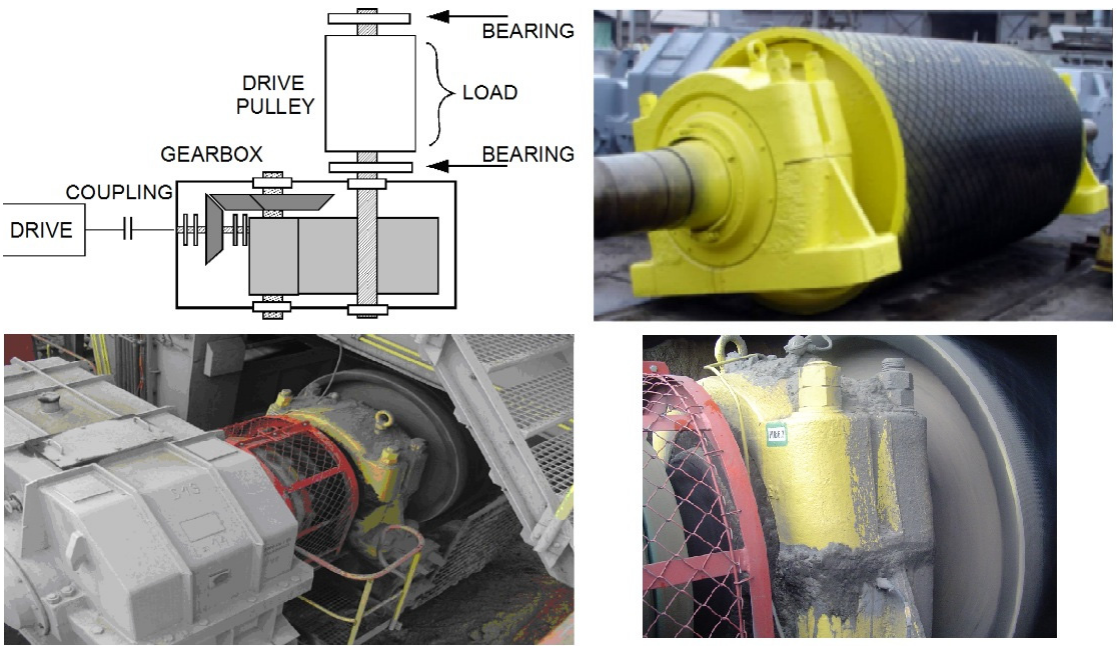
\includegraphics[width=0.9\textwidth]{wykresy/gb.PNG}
\caption{Rolling bearing location in~the~driving station}
\label{fig:gb}
\end{figure}

Fig. \ref{fig:gb} presents the~schematic of~the~drive unit for a~belt conveyor with the~indication where the~bearings are operating. The drive unit consists of~an~electric motor, a~coupling and two stage gearbox, that are connected with a~pulley.

\begin{table}
\begin{center}
	\begin{tabular}{|c|l|l|l|}
		\hline
		No & Notation & Description & Value/unit \\ \hline
		1 & $f_{FTF}$ & Fundamental train frequency & 0.51 Hz \\ \hline
		2 & $f_{BSF}$ & Ball spin frequency & 4.45 Hz \\ \hline
		3 & $f_{BFF}$ & Ball fault frequency & 8.9 Hz \\ \hline
		4 & $f_{BPFO}$ & Ball passing frequency outer race & 12.69 Hz \\ \hline
		5 & $f_{BPFI}$ & Ball passing frequency inner race & 16.06 Hz \\ \hline
		
		%\caption{Bearing frequencies: 23264 CCK/W33}
	\end{tabular}
\end{center} 
\caption{Bearing frequencies: 23264 CCK/W33}
\label{loz_table}
\end{table}


% The pulley consists of~a~shaft, two bearings and the~coating covered by~rubber (to increase friction between the~pulley coating and the~belt). Often between the~gearbox and the~pulley a~rigid coupling is~used.
\subsubsection{Experiment}

Several measurements have been conducted using Pr{\"u}ftechnik online measurement system. For each measurement the~signal was acquired with the~ sampling frequency $f_s = 19.2$ kHz and duration T = 2.5 s. Fault of~the~investigated bearing has been identified as~a~local damage on~the~outer race.

\subsection{Reciprocating gas compressor}

The studied machine is~a~1000 kW reciprocating gas compressor of~a~type Dresser-Rand C-VIP, operating between 600-1000 rpm, with a~four-stage compression \cite{barszcz2013bearings}. The machine operates on~the~offshore oil rig. The key issue is~that vibration signals generated by~the~compressor contain a~number of~external disturbances, the~most influential being the~piston-related and valve-related ones. 

\begin{table}[ht!]
  \centering
  \caption{Machine-related frequencies for investigated compressor}
  \begin{tabular}{|l|l|}
  \hline
     \textbf{Parameter} & \textbf{Frequency [Hz]} \\ \hline
     Sampling frequency & 24000 \\ \hline
     Shaft speed & 12.35 \\ \hline
     BPFI & 127.9 \\ 
  \hline
  \end{tabular}
  \label{tab:tab1}
\end{table}

\begin{figure}[ht!]
\centering
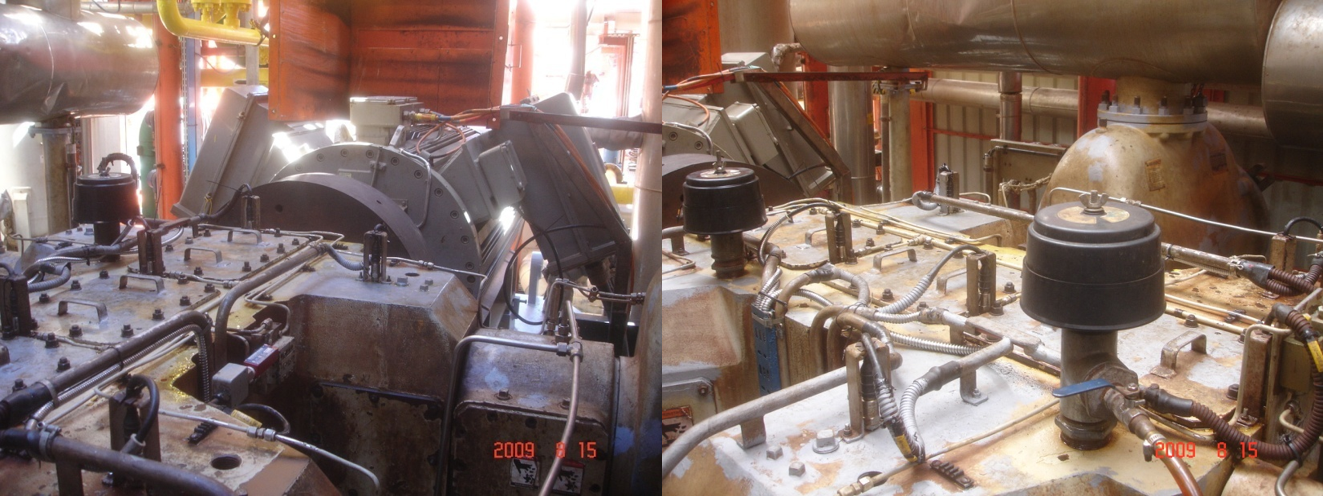
\includegraphics[width=0.8\textwidth]{wykresy/obj_komp.png}
\caption{Reciprocating gas compressor operating on~the~oil rig}
\label{fig:obj_komp}
\end{figure}

\subsubsection{Experiment}

Vibration measurement has been performed using on-board live monitoring system with sampling frequency $f_s=24$ kHz. It has been discovered that the~analyzed signal has been recorded when the~inner ring has been severely defected in~one of~the~main shaft bearings. Details including the~SOI parameters are presented in~Table~\ref{tab:tab1}.

\subsection{Copper ore crusher in~mineral processing plant}

The machine under investigation is~a~copper ore hammer crusher operating in~mineral processing plant (see Figure \ref{fig:obj_crusher}). Analysis of~vibration signal measured on~such machine is~very challenging from the~signal processing point of~view. The difficulty lies in~the~way that the~machine operates. Rock pieces falling into the~machine from the~top hit the~walls in~a~random way, which generates very strong impulses. Similar impulses are caused by~the~hammers crushing the~pieces. In terms of~stochastic modeling it~is~a~non-Gaussian noise. It is~described as~a~noise because it~occurs randomly, and it~is~non-Gaussian, because it~has relatively high probability of~high values not associated with Gaussian distribution, that manifest as~mentioned impulses. Considering the~presence of~such noise it~is~very difficult to~be able to~detect modulations related to~damage on~one of~the~elements, because corresponding cyclic component is~expected to~also be~impulsive, but much less energetic.

\begin{figure}[ht!]
\centering
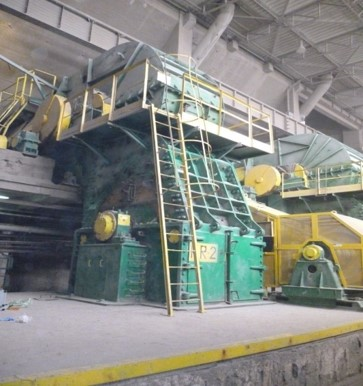
\includegraphics[width=0.5\textwidth]{wykresy/obj_crusher.jpg}
\caption{Copper ore crusher}
\label{fig:obj_crusher}
\end{figure}

\begin{table}
	\begin{center}
\begin{tabular}{|c|l|l|l|}
	\hline
   No & Notation & Description & Value/unit \\ \hline
	1 & $n_i$ & Rotational speed of~the~inner ring & 180 RPM \\ \hline
	2 & $F_i$ & Rotational frequency of~the~inner ring & 3 Hz \\ \hline
	3 & $F_c$ & Rotational freq. of~the~rolling element and cage assembly & 1.3 Hz \\ \hline
	4 & $F_r$ & Rotational freq. of~a~rolling element about its own axis & 10.6 Hz \\ \hline
	5 & $F_{ip}$ & Over-rolling frequency of~one point on~the~inner ring & 30.7 Hz \\ \hline
	6 & $F_{ep}$ & Over-rolling frequency of~one point on~the~outer ring & 23.3 Hz \\ \hline
	7 & $F_{rp}$ & Over-rolling frequency of~one point on~a~rolling element & 21.1 Hz \\ \hline
\end{tabular}
\end{center} 
\caption{Bearing frequencies from copper ore crusher}
\label{krusz_table}
\end{table}

\subsubsection{Experiment}
The considered element was 23264 SKF bearing. Vibration data has been measured in~two orthogonal directions with Endevco accelerometers, and signal acquisition was based on~NI-DAQ card and LabView Signal Express environment. Sampling frequency of~vibrations signals is~25 kHz. The particular vibration signal considered in~this dissertation is~a~10-second section of~the~60-second measurement session. Characteristic frequencies of~the~bearing are presented in~Table \ref{krusz_table}. Fault of~the~investigated bearing has been identified as~a~local damage on~the~inner race.


\section{Objects of~interest for analysis of~other types of~data}
 
Vibration data analysis is~a~very important component of~this dissertation, however it~is~not the~only type of~data under investigation. Hence, in~this section author describes the~machines that have provided other types of~data. This group contains the~gearbox of~conveyor belt drive and self-propelled load-haul-dump wheeled machine (LHD). 

\subsection{Load-Haul-Dump machines in~underground mine}

Load-haul-dump machines (LHD, a.k.a. \emph{loaders}, see Figure \ref{fig:obj_lhd}) are key assets used in~Polish copper ore mines. They are designed to~load blasted ore from mining face onto haulage trucks, or transport ore to~the~screen by~themselves. Reliability and effectiveness of~those machines have a~huge impact on~the~overall performance of~the~production. LHD machines along with their maintenance are also one of~the~most expensive aspects of~underground mining. Strongly time-varying and harsh operating conditions determine high workload, that in~connection with high effectiveness and availability demands are a~big challenge for maintaining their technical condition on~the~highest level possible.

\begin{figure}[ht!]
\centering
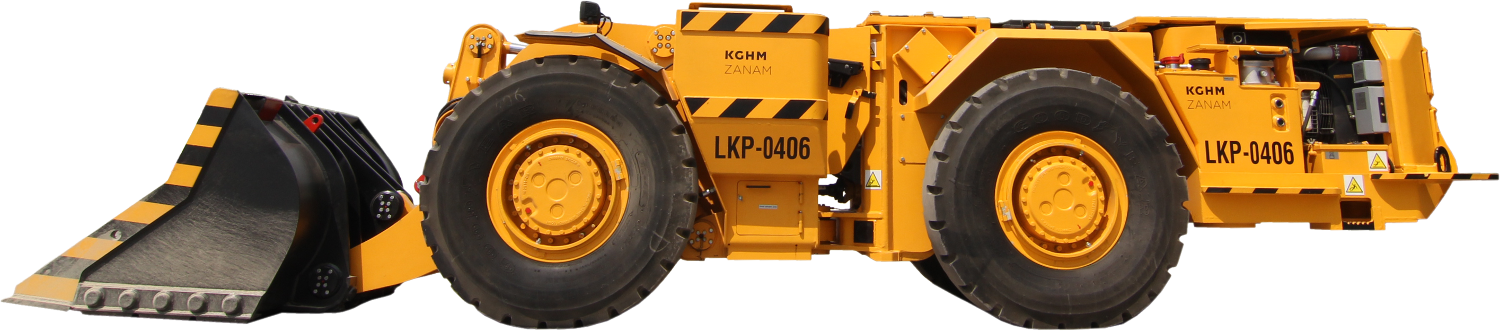
\includegraphics[width=\textwidth]{wykresy/obj_lhd.png}
\caption{Self-propelled Load-Haul-Dump machine}
\label{fig:obj_lhd}
\end{figure}

One of~the~most important problems of~those machines is~overheating, hence temperature data recorded from LHD-s is~very important in~the~condition monitoring process. However during the~operations of~loading temperature itself strongly varies, which is~closely related to~technical condition, operating load and harsh mining conditions, but also the~fact that the~machine can perform various tasks and take different route during every work shift. In this case the~analysis of~temperature data is~very difficult especially in~the~long term, because there is~virtually no control over the~details of~the~process from the~point of~view of~data acquisition being interpreted as~an~experiment. 

\subsubsection{Experiment}
Diagnostic data is~registered using on-board acquisition system installed by~the~manufacturer. Beside the~engine coolant temperature analyzed in~this dissertation there is~a~lot of~other parameters being registered on~the~LHDs, including but not limited to:
\begin{itemize}
  \item pressures of~engine oil, gearbox oil, oil in~hydraulic actuation system etc.,
  \item temperatures of~engine oil, gearbox oil, oil in~hydraulic actuation system etc.,
  \item rotations per minute of~the~engine shaft,
  \item speed of~the~vehicle.
\end{itemize}

Individual parameters can be~sampled with different frequencies, but for the~purpose of~saving the~storage space all of~sampling frequencies are set by~default to~1 Hz. In case of~certain parameters describing fast-changing processes it~could be~a~disadvantage, however, since temperature is~a~case of~slowly-changing process with inherent inertia, analytical methodology does not suffer from the~relatively slow sampling. Moreover, such configuration allows to~store records from the~entire lifetime of~the~machine in~the~databases of~the~owning company.

In case of~the~analyses presented further in~this dissertation author uses the~variable describing the~temperature of~the~engine coolant, further referred to~as \emph{temperature data}. Available record spanned over the~period of~2,5 months. During this period the~machine was performing tasks typical for its purpose, such as~picking up blasted material from the~mining face and transporting it~to~the~dumping screen in~case of~operating on~its own, or dumping the~material to~the~bucket of~haulage truck in~case of~work in~conjunction.

\subsection{Gearbox in~underground belt conveyor drive}

Vibration data is~generally considered to~be a~better source of~diagnostic information than temperature for many reasons:

\begin{itemize}
  \item the~information about occurring events is~instantaneous,
  \item signal has broader bandwidth, hence it~is~richer in~useful components,
  \item all the~information is~aggregated, and in~practice impossible to~be decomposed in~a~way that vibration data can be, because of~the~insufficient bandwidth.
  \item it~is~possible to~observe processes much weaker in~energy that are not manifesting themselves in~the~temperature data etc.
\end{itemize}

Unfortunately, it~is~not always possible to~obtain it. In most cases machines are not equipped with built-in vibration acquisition system, and to~perform the~measurement it~is~necessary to~send a~person equipped with a~portable measurement system. On the~other hand, much more machines have built-in capability to~record temperature data because of~the~installed monitoring systems.

In many cases failures of~gearboxes are manifested by~overall machine overheating. However gearboxes operating in~belt conveyor drives, as~well as~belt conveyors as~a~whole, can be~considered as~time-varying system and direct decision making using direct readout of~parameters can be~very difficult. To address this issue, long-term analysis of~records such as~temperature enables to~learn how to~recognize alarming moment. Thus the~maintenance tasks can be~better scheduled to~minimize the~stoppages and losses in~production. 

\subsubsection{Experiment}
Temperature is~measured on~gearbox casing using SCADA system used continuously by~the~mining company. Data sampling is~not fixed, the~next sample is~recorded when the~temperature exceeds predefined resolution threshold with respect to~the~previous sample. Such approach allows to~use less storage space for the~registered data. However, many analytical techniques require even data sampling, so resampling procedures are very often a~necessary preprocessing step for such data.

In case of~temperature record analyzed in~this dissertation, data spans over the~period of~72 days, when the~machine was operating in~its typical manner described described more in~section \ref{temp_em}. 